\begin{ledgroupsized}[r]{120mm}
\footnotesize
\pstart
\noindent
\textbf{\"{U}berlieferung:}
\pend
\end{ledgroupsized}
\begin{ledgroupsized}[r]{114mm}
\footnotesize
\pstart
\parindent -6mm
\makebox[6mm][l]{\textit{L}}%
Aufzeichnung: LH XXXVII 3 Bl. 16. 1 Bl. 4\textsuperscript{o}.
1 S. auf Bl. 16~r\textsuperscript{o}. Bl. 16~v\textsuperscript{o} leer.
Zwei gestrichene Ansätze zu einer Zeichnung werden nicht wiedergegeben.\\%
Cc 2, Nr. 485
\pend
\end{ledgroupsized}
%\normalsize
\vspace*{4mm}
\begin{ledgroup}
\footnotesize
\pstart
\noindent
\footnotesize{\textbf{Datierungsgr\"{u}nde:} Magnetismus und magnetische Missweisung stehen in Zusammenhang mit dem Problem der geographischen Längengradbestimmung. Auf diesen Zusammenhang gehen die Stücke \cite{01072}\textit{LSB} VIII, 1 N. $6_1$ und N. $6_2$ ein,
deren Datierung hier übernommen wird.}
\pend
\count\Afootins=1500
\count\Bfootins=1000
\count\Cfootins=1500
\end{ledgroup}
\vspace*{4mm}
\pstart%
\normalsize%
\noindent%
[16~r\textsuperscript{o}]\\
$AB$ aiguille.
\pend
\pstart%
\noindent%
$CD$ distance de laquelle 
l'aiguille\protect\index{Sachverzeichnis}{l'aiguille} $AB$ est tirée
\hspace{2mm}
par les deux poles tout à la fois,
\pend
\pstart\noindent
\hspace{74mm} chacun tirant son bout. \\
$CE$ \textso{ ..............................}
\hspace{9mm}par un pole seulement.
\pend
\pstart%
\noindent%
\textit{IK} aiguille plus longue et plus epaisse que la premiere \textit{AB}.
\newline%
\textit{FG} la distance de laquelle l'aiguille \textit{IK} est attir\'{e}e depuis son support \textit{LM} jusques à \textit{NP}.
\newline%
\textit{NP} est le cost\'{e} d'Est ou Ouest  (\textit{Q} \edtext{longueur de la piece}{\lemma{longueur de la piece}\Bfootnote{\textit{erg. L}}} est Sud ou Nord[).]
\newline%
\textit{SRT} est le bas de l'aimant\protect\index{Sachverzeichnis}{l'aimant}
\edtext{(mais qui est erig\'{e} icy),}{\lemma{(mais [...] icy)}\Bfootnote{\textit{erg. L}}}
et \textit{ST}, les armatures.
\newline%
\textit{GH} est egale \`{a} \textit{NS} distance des armatures\protect\index{Sachverzeichnis}{armature} \edtext{de l'extremit\'{e}}{\lemma{armatures}\Bfootnote{\textit{(1) }\ du cost\'{e} \textit{(2)}\ de l'extremit\'{e} \textit{L}\ }} de la boette.
\pend
\pstart%
Je remarque qu'une aiguille peut estre attir\'{e}e de la distance \textit{FGH} \edtext{ou \textit{LS}.}{\lemma{ou \textit{LS}}\Bfootnote{\textit{erg. L}}}
Car premierement elle est attir\'{e}e de \textit{F} en \textit{G}, c'est \`{a} dire de \textit{L} en \textit{N} par apr\`{e}s si on \edtext{[l']}{\lemma{}\Bfootnote{l'on\textit{\ L \"{a}ndert Hrsg.}}}empeche de s'y attacher au cost\'{e} \textit{NP}, ou de rencontrer un angle ou autre obstacle; elle montera jusqu'en \textit{S} aux armatures.  
\pend 
\pstart Soit la cheville $\alpha$, qui glisse un peu sur la regle $\alpha \beta$, et en $\beta$ monte par l'arc $\beta \gamma$ jusqu'\`{a} l'armature \textit{S}.  
\pend
\pstart  Car en luy donnant une planche bien unie sans arc en inclinant une regle de coton\protect\index{Sachverzeichnis}{coton} au lieu de $\beta \gamma$, l'aiguille est \edtext{souuent}{\lemma{souuent}\Bfootnote{\textit{erg. L}}} mont\'{e}e.
\pend
\pstart
J'ay remarqu\'{e} qu'une aiguille \edtext{rougie, n'est pas moins attir\'{e}e pour cela.}{\lemma{rougie,}\Bfootnote{\textit{(1)}\ ne perd pas par la \textit{(2)}\ n'est [...] cela \textit{L}}}
Item qu'il est difficile d'augmenter la distance ou sphere d'activit\'{e} mais qu'on peut augmenter la pesanteur de l'aiguille qui doit estre tir\'{e}e. 
\pend
\newpage
\pstart
\centering
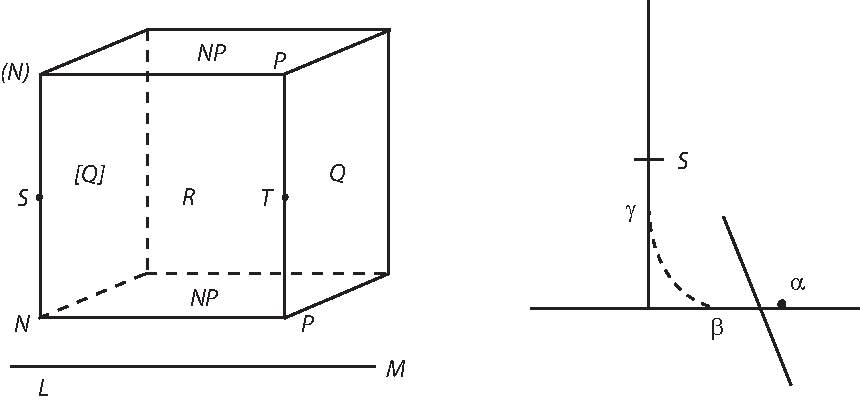
\includegraphics[width=0.9\textwidth]{images/37316r_fig23.pdf}\\
\vspace*{0.5mm}\hspace*{10mm}[\textit{Fig. 1}] \hspace*{60mm} [\textit{Fig. 2}]
\pend
\vspace{2.5em}
\pstart 
\advanceline{-2}Car ayant joint deux aiguilles comme \textit{AB} en une \textit{VX}, et ayant encor adjout\'{e} beaucoup 
de cire, l'aymant\protect\index{Sachverzeichnis}{l'aymant} l'a neantmoins tir\'{e} d'une distance, qui n'estoit pas plus petite de beaucoup, qu'auparavant.
\pend
\pstart
Posons qu'une telle aiguille\protect\index{Sachverzeichnis}{l'aiguille} pese un grain ou quelque chose d'avantage, la double aiguille deux ou trois, et la cire\protect\index{Sachverzeichnis}{cire} adjout\'{e}e en pesoit bien 5 ou six. La longueur d'une aiguille nuira pas, si on la fait attirer par les deux poles tout \`{a} la fois; et si  les poles aussi sont fort distans les uns des autres. Je remarque qu'une aiguille\protect\index{Sachverzeichnis}{l'aiguille} pli\'{e}e en une masse est difficilement attir\'{e}e.
\pend
\vspace{2em}
\count\Afootins=1500
\count\Bfootins=1500
\count\Cfootins=1500
\pstart
\advanceline{-2}
\centering
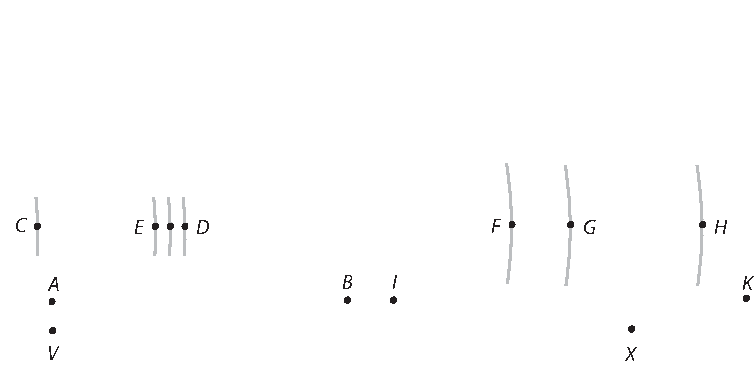
\includegraphics[trim = 0mm 0mm -3mm 25mm, clip, width=1.0\textwidth]{images/37316r_fig1.pdf}\\
\vspace*{0.5mm}\centering [\textit{Fig. 3}]
\pend